\documentclass[12pt,letterpaper]{article}
\usepackage[utf8]{inputenc}

%Documento
\usepackage[spanish,es-tabla,es-lcroman]{babel}
\usepackage[T1]{fontenc}
\usepackage{times}
\usepackage[margin=2.54cm]{geometry}
\usepackage{parskip} %saltos de parrafo
\setlength{\parskip}{\baselineskip}

%Formatos
\usepackage{setspace} %espacios de interlineados
\usepackage[dvipsnames]{xcolor} %paquete para colores
%tablas
\usepackage{array}
\usepackage{multicol}
\usepackage{longtable}

%imagenes
\usepackage{graphicx}
\usepackage{subcaption}
\usepackage{enumerate} %numeracion de tablas y figuras
%Listas
\usepackage[shortlabels]{enumitem}

%hipervinculos
\usepackage{hyperref}%Genera hipervinculos
\hypersetup{colorlinks=true,citecolor=black,filecolor=black,linkcolor=black,urlcolor=blue}

%Referencias
\usepackage{natbib}

%matematicas
\usepackage{amsmath,amssymb,amsfonts}

% - - - - - - - - - - - - - - - - - - - - - - - - - - - - - - - - - - - - - - - - - - - - - - 
%Indice de ecuaciones, figuras y tablas
\numberwithin{equation}{section} 	
\numberwithin{figure}{section}
\numberwithin{table}{section}

\begin{document}
\begin{titlepage}
    \begin{center}
        \noindent 
\includegraphics[width=\textwidth]{Imagenes/logos latex.PNG} \\[2cm] %el noident fue para quitar la sangria... texwidht es para que la imagen sea del ancho de la pagina 
        \textbf{{\Huge CENTRO NACIONAL DE INVESTIGACIÓN Y DESARROLLO TECNOLÓGICO}}\\[1cm]
        
        \textbf{\Large{Doctorado en Ciencias en Ingeniería Electrónica}}\\
        {\large Especialidad en Control Automático}\\[1cm]
        
        \textbf{{\Large Propuesta de tesis}}\\
        {\large 2° semestre}\\[1cm]
              
        \textbf{\Large{\textcolor{MidnightBlue}{Modelado de datos ómicos con técnicas de aprendizaje profundo mediante redes neuronales}}}\\[1cm]
        
        {\large Presenta:}\\
        \textbf{{\Large M.C. Arturo Figueroa Arcos}}\\[1cm]
    
    \end{center}
    \begin{minipage}{0.46\textwidth}								
        \begin{flushleft}
        \begin{center}
    
            \textbf{Directores de tesis:}\\
        
            Dr.\ Víctor Manuel Alvarado Martínez\
            Dra. Ma. Guadalupe López López\\
            
    \end{center}
    \end{flushleft}
    \end{minipage}		
                                                                    %%%
    \begin{minipage}{0.52\textwidth}		
    \vspace{0cm}
    \begin{flushright}															%%%
    \begin{center}
    
            \textbf{Revisores de tesis:}\\
    
            Dr.\ Luis Gerardo Vela Valdés\\
            Dr.\ Victor Hugo Olivares Peregrino\\
            Dra. Marisol Cervantes Bobadilla\\
    
            
    \end{center}
    \end{flushright}
    \end{minipage}	
    \vspace*{3cm}
    
    \begin{flushright}
    {\large Cuernavaca, Morelos a 06 de diciembre de 2024}
    \end{flushright}
    
    \end{titlepage}
\pagenumbering{roman}
\renewcommand{\contentsname}{Tabla de contenido}
\tableofcontents
\newpage

\newpage
\listoffigures
\addcontentsline{toc}{section}{Índice de figuras}

\newpage
\listoftables
\addcontentsline{toc}{section}{Índice de tablas}

\newpage
\addcontentsline{toc}{section}{Nomenclatura}

% - - - - - - - - - - - - - - - - - - -- - - - - - - - - - - - - - - - - - - - - - - -- - - - -
%Nomenclatura

\textbf{\Large{Nomenclatura}}

\begin{table}[h]

    \centering
    \caption{Siglas y acrónimos}
    \vspace{0.3cm}
    \begin{tabular}{
    >{\centering\arraybackslash}m{3cm}
    >{\centering\arraybackslash}m{12cm}} \hline

\textbf{Siglas} & 
\textbf{Descripción} \\ \hline\hline

    IA & Inteligencia Artificial
\\[0.2cm]

   DL & Deep Learning
\\[0.2cm]

   ML & Machine Learning 
\\[0.2cm]

   CNN & Convolutional Neuronal Network
\\[0.2cm]
   RNN & Recurrent Neuronal Network 
\\[0.2cm]
   NGS & Next Generation Sequencing 
\\[0.2cm]
   ANN & Artificial Neuronal Network 
\\[0.2cm]

\hline
    \end{tabular}
\end{table}

\newpage

\setcounter{page}{1} %se reinicia el contador de la páginas después de la Tabla de contenido
\pagenumbering{arabic}

% - - - - - - - - - - - - - - - - - - - - - - - - - - - - - - - -
%Documento principal

\section{Introducción}

En la ingeniería biomédica se aplica tecnología de última generación, para la creación de dispositivos médicos y métodos que permitan contribuir al bienestar humano, para obtener una mejora en la compresión de los procesos biológicos que suceden en el ser humano. En este campo de estudio intervienen áreas como la ingeniería electrónica, la ingeniería mecánica, la medicina, la biología, la física, entre otros, considerando a la ingeniería biomédica como un campo interdisciplinario.

La generación de datos ómicos ha experimentado un crecimiento exponencial gracias a las tecnologías de secuenciación de alto rendimiento (NGS). Debido a la alta cantidad de datos existentes, se han impulsado métodos analíticos avanzados para interpretarle y extraer información biológica significativa. Los datos que se abarcan son de diferentes niveles de organización molecular, como el ADN, el ARN, las proteínas y metabolitos.

 Algunos ejemplos de estos datos ómicos son los genómicos que estudian el ADN incluyendo la secuencia, estructura y función, los datos transcriptómicos que estudian el ARN incluyendo su expresión, splicing y modificaciones, los datos proteómicos que estudian las proteínas, incluyendo su estructura, función e interacciones y los datos metabolómicos que estudian las moléculas pequeñas que interactúan en las reacciones químicas de la célula.

El análisis de este tipo de datos cuenta con el potencial para mejorar significativamente nuestra compresión de la salud y las enfermedades en un ser humano. Los pasos típicos son el preprocesamiento donde se realiza la limpieza y normalización de los datos con el fin de eliminar errores, control de calidad para identificar y eliminar posibles valores atípicos, análisis estadístico para identificar biomarcadores relevantes así como también modelos predictivos y de asociación y por último la interpretación de los resultados con sentido biológico.
Algunos de los desafíos que se presentan en el análisis son el alto volumen de datos, complejidad de los datos y la integración de tipo de datos, es por ello por lo que se considera un desafío computacional.

El Aprendizaje Profundo (DL) es un campo de la inteligencia artificial, que ha demostrado ser una herramienta poderosa para el análisis de datos complejos, está basado en la utilización de redes neuronales artificiales (ANN’s) con el fin de identificar patrones complejos, realizar análisis no lineales y modelar relaciones a partir de diferentes tipos de datos ómicos.

Las ANN’s y DL aplicadas en la ingeniería biomédica representan una oportunidad para los profesionales de la salud, ya que permiten realizar análisis más rápidos de grandes conjuntos de datos e información médica relevante, mejoras en los métodos de diagnóstico y pronostico de enfermedades, diseño de terapias personalizadas y mejoras para el bienestar humano. Los principales desafíos que se presentan son la necesidad de grandes conjuntos de datos para entrenamiento de las redes, la interpretabilidad de las redes neuronales para comprender su toma de decisiones y el requerimiento computacional para entrenamiento de las redes \citep{sarmiento2020aplicaciones}.

En este proyecto se enfocará con el propósito de clasificación de tipos y subtipos de fenotipos, así como también en el pronóstico de supervivencia, utilizando de manera preliminar datos ómicos centrados en el cáncer como los genómicos, transcriptómicos, proteómicos y metabolómicos. El área de oportunidad que se encuentra es en el preprocesamiento de datos y la codificación debido a la heterogeneidad de los datos procedentes de distintas bases que se encuentran de libre acceso. El propósito de este estudio estará dirigido en el estudio de algoritmos de aprendizaje profundo e implementarlos con enfoque de aplicación en el área biomédica con el fin de dar soporte en la precisión del diagnóstico y predicción de enfermedades.
\section{Marco conceptual}

\subsection{Datos ómicos}

Las ciencias ómicas conocidas también como biomedicina o bioinformática, estudian los procesos biológicos a nivel molecular a través de grandes conjuntos de datos con el fin de diagnosticar, prevenir y predecir enfermedades, así como también en terapias y tratamientos personalizados en pacientes. El término de “omica” se deriva del griego "óma" que significa masa o conjunto \citep{ravi2016deep,mamoshina2016applications}. La omica es un campo de la biomédica con una gran extensión y esta se divide en diferentes ramas como la genómica, transcriptómica, proteómica, metabolómica, epigenómica, farmacogenómica y metagenómica.

\subsection{Tipos de ciencias ómicas}

Las diferentes ramas de la ómica se dirigen a distintos niveles moleculares, habitualmente se estudian de manera independiente a la hora de abordar enfermedades y obtener conocimiento médico y científico, cada una ofrece información importante, pero en conjunto las ciencias permiten obtener relaciones de los niveles moleculares y entender su complejidad biológica (Figura~\ref{fig:tip_omic})

\begin{figure}[h!]
    \centering
    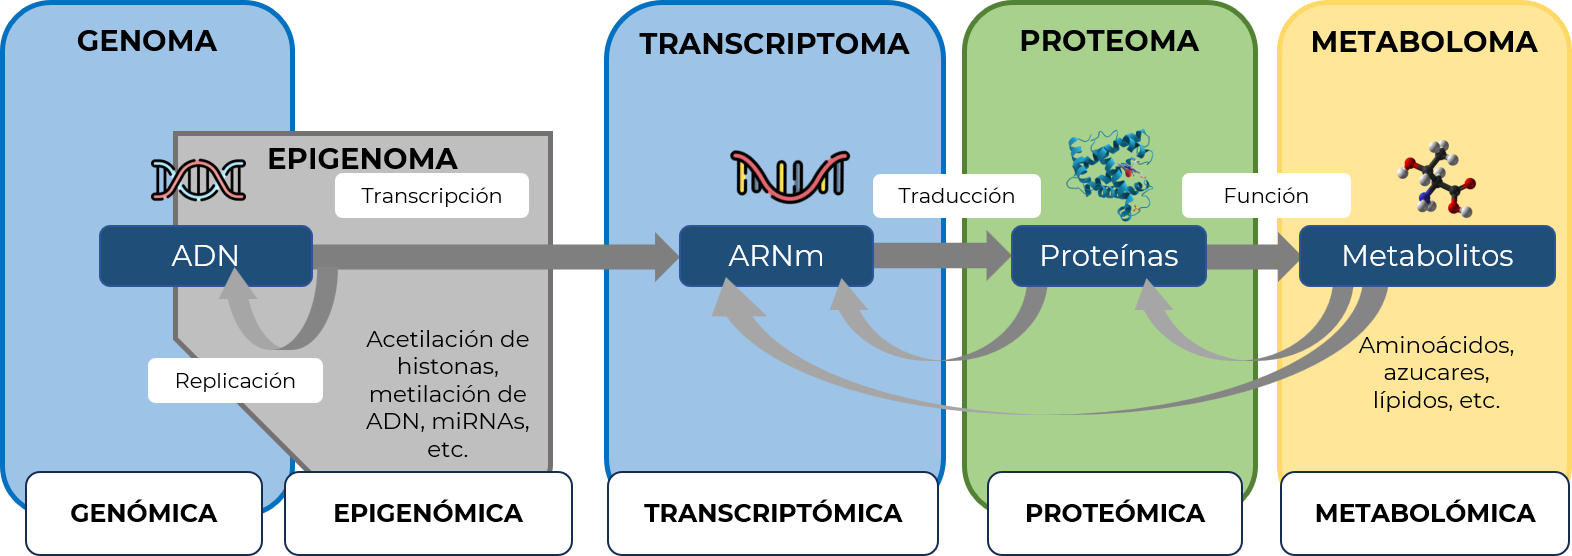
\includegraphics[width=0.9\textwidth]{Imagenes/Tip_omic.png}
    \caption{Clasificación de ciencias ómicas y relación entre ellas}
    \label{fig:tip_omic}
\end{figure}



La genómica es de las primeras ciencias ómicas en reconocerse como tal, esta se encarga del estudio de los genomas, es decir, la totalidad del material genético que tiene un organismo vivo o una partícula viral. El objetivo es identificar alelos genéticos y factores ambientales que contribuyen al desarrollo de enfermedades \citep{institute}.

La transcriptómica estudia el patrón de la expresión genética en un organismo o en células específicas bajo circunstancias concretas, es decir, el conjunto de los ARN mensajeros (ARNm) y no codificantes, a nivel cuantitativo y cualitativo \citep{davis2017missing}.

La epigenómica estudia el conjunto de modificaciones reversibles del ADN o de las proteínas asociadas al ADN (como las histonas) que actúan como elementos funcionales de regulación de la expresión génica de una célula sin alterar la secuencia de su ADN \citep{hasin2017multi}.

La proteómica estudia el conjunto de las proteínas con sus isoformas y modificaciones postraduccionales expresadas en una celular, tejido u órgano concreto en un momento dado, bajo determinadas condiciones y localización específica, dado que las proteínas median las actividades bioquímicas en una célula \citep{van2018precision}.

La metabólica es la ciencia que estudia el conjunto completo de los metabolitos (intermediarios metabólicos, hormonas y metabolitos secundarios) que se encuentran en un momento dado en una célula, tejido u órgano. Entre los metabolitos estudiados se incluyen desde el oxígeno, los aminoácidos esenciales o las vitaminas \citep{zhao2014lipidomics}.

En la tabla~\ref{tab:List_omic} siguiente se resume la información de las ciencias ómicas establecidas y su definición por área de estudio:

\begin{table}[!h]
    \scriptsize
    \centering
    \caption{Listado de ciencias ómicas establecidas}
    
    \begin{tabular}{
    >{\centering\arraybackslash}m{4cm} 
    >{\centering\arraybackslash}m{9cm}}
\hline 
        \textbf{Ciencia ómica} & 
        \textbf{Área de estudio}
\\      
    \hline \hline 

    Genómica &
    Estudio del conjunto del material genético presente en un organismo.
\\
    \hline
    Transcriptómica &
    Estudio de los perfiles de expresión de los ARN mensajeros, los microARNS y ARN no codificantes.
\\
    \hline
    Epigenómica &
    Estudio de los elementos que controlan la expresión génica sin modificar la secuencia de nucleótidos del ADN.
\\
    \hline
     Proteómica &
     Estudio del set completo de proteínas expresadas en un organismo en un tiempo determinado y particular de cada tipo celular o tisular.
\\
     \hline
     Metabolómica &
     Identificación y cuantificación de productos metabólicos de pequeño tamaño (metabolitos) de un sistema biológico (célula, tejido, fluido biológico u órgano)
\\
     \hline
     Farmacogenómica &
     Estudio de los genes que afectan a la respuesta de una persona a determinados fármacos
\\
     \hline
     Metagenómica &
     Estudio del conjunto de microorganismos de una muestra ambiental para proporcionar información de la diversidad ecológica de un ambiente determinado.
\\
    
\hline
    \end{tabular}
    \label{tab:List_omic}
\end{table}

\subsection{Representación de datos ómicos}

En cada ciencia ómica se tiene un tipo distinto de representación de acuerdo al tipo de datos que se extraen, esto es fundamental para el almacenamiento, análisis e interpretación de este tipo de datos, para permitir a los investigadores extraer características biológicas, en la Tabla~\ref{tab:Datos_cod} se muestra la forma en que se representa cada dato:

\begin{table}[!h]
    \scriptsize
    \centering
    \caption{Representación de los datos más frecuentemente utilizados}
    
    \begin{tabular}{
    >{\centering\arraybackslash}m{4cm} 
    >{\centering\arraybackslash}m{9cm}}
\hline 
        \textbf{Tipos de datos} & 
        \textbf{Descripción de la representación} 
\\      
    \hline \hline 

    Genómicos &
    Secuencias de ADN, representadas por cadenas de 4 caracteres.
\\
    \hline
    Transcriptómicos &
    Perfiles de expresión genética, representados por una tabla o matriz numérica.
\\
    \hline
    Epigenómicos &
    Señales registradas en un vector que contiene series temporales o perfiles, representadas en una tabla de valores numéricos.
\\
    \hline
     Proteómicos &
     Secuencias de proteínas, representadas por una cadena de 20 caracteres. Espectrometría de masas, representada por un vector con serie temporal.
\\
     \hline
     Metabolómicos &
     Cálculo de espectro, representado por vector con series temporales.
     Perfiles, representados en una tabla con valores numéricos.
\\
    
\hline
    \end{tabular}
    \label{tab:Datos_cod}
\end{table}

\subsection{Redes neuronales artificiales}
%Fuente: https://doi.org/10.18273/revuin.v19n4-2020001

 Las ANN son un modelo de algoritmo computacional inspirado en las redes biológicas, con el que se establecen relaciones entre las entradas y salidas. Se caracteriza por ser una herramienta que tiene la capacidad para aprender, procesar y generalizar automáticamente datos, utilizadas en tareas de clasificación y regresión \citep{NeuronalNet2014}. En el propósito de clasificación, los datos de entrada son clasificados en distintas clases, y en la regresión, o aproximación de función, se realiza para predecir un parámetro de salida desconocido \citep{NeuronalNet2014}. Es por esto que las ANN cuentan con el potencial en aplicaciones de reconocimiento de patrones y predicción de comportamiento.

 \subsubsection{Componentes de la red neuronal}

 Una neurona artificial se compone de una o múltiples entradas $p$, un peso $w$, un bias o umbral $b$, un sumador $\sum$ y una función de activación $f$, como se puede observar en la Figura~\ref{fig:Neu_Diag}. 

 \begin{figure}[!h]
     \centering
     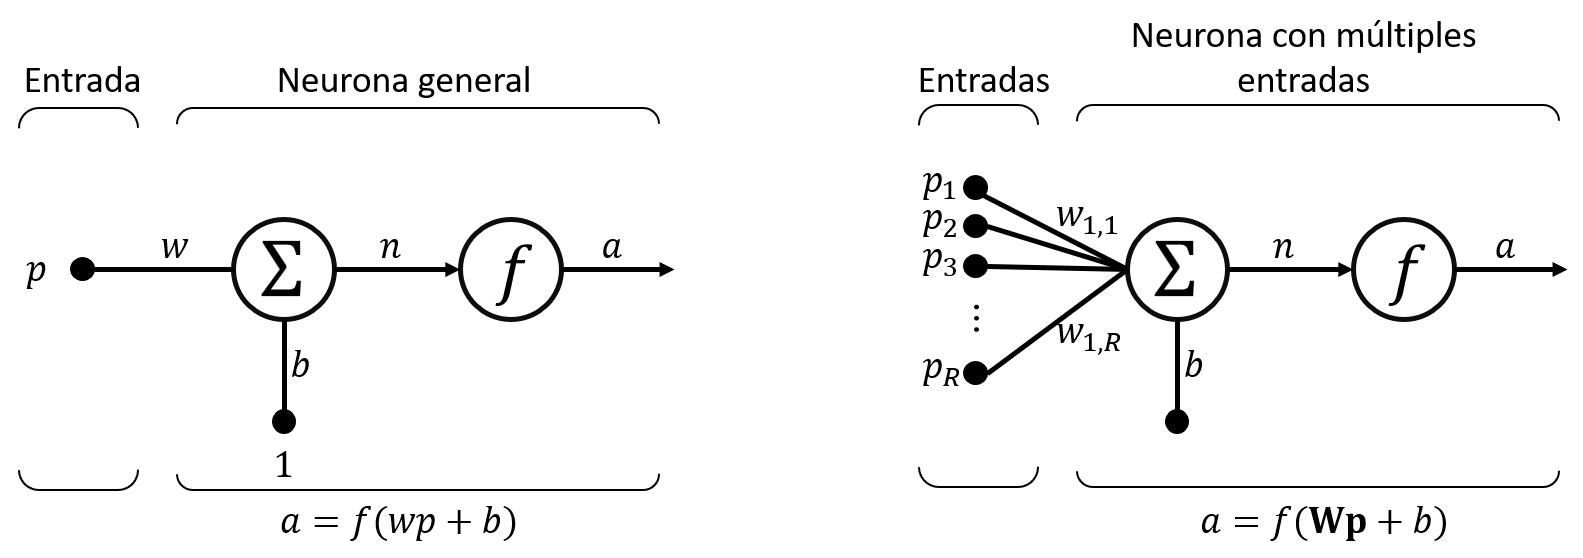
\includegraphics[width=0.8\textwidth]
     {Imagenes/Neu_Diag.png}
     \caption{Representación de neuronas artificiales de una entrada y múltiples entradas \citep{NeuronalNet2014}.}
\label{fig:Neu_Diag}
 \end{figure}

 Normalmente, una neurona con múltiples entradas suele no ser suficiente, por lo que las ANN se usan con varias neuronas ubicadas en paralelo formando un “capa”. Las ANN pueden poseer una capa o múltiples como se observa en la Figura~\ref{fig:Net_conjunt}.

  \begin{figure}[!h]
     \centering
     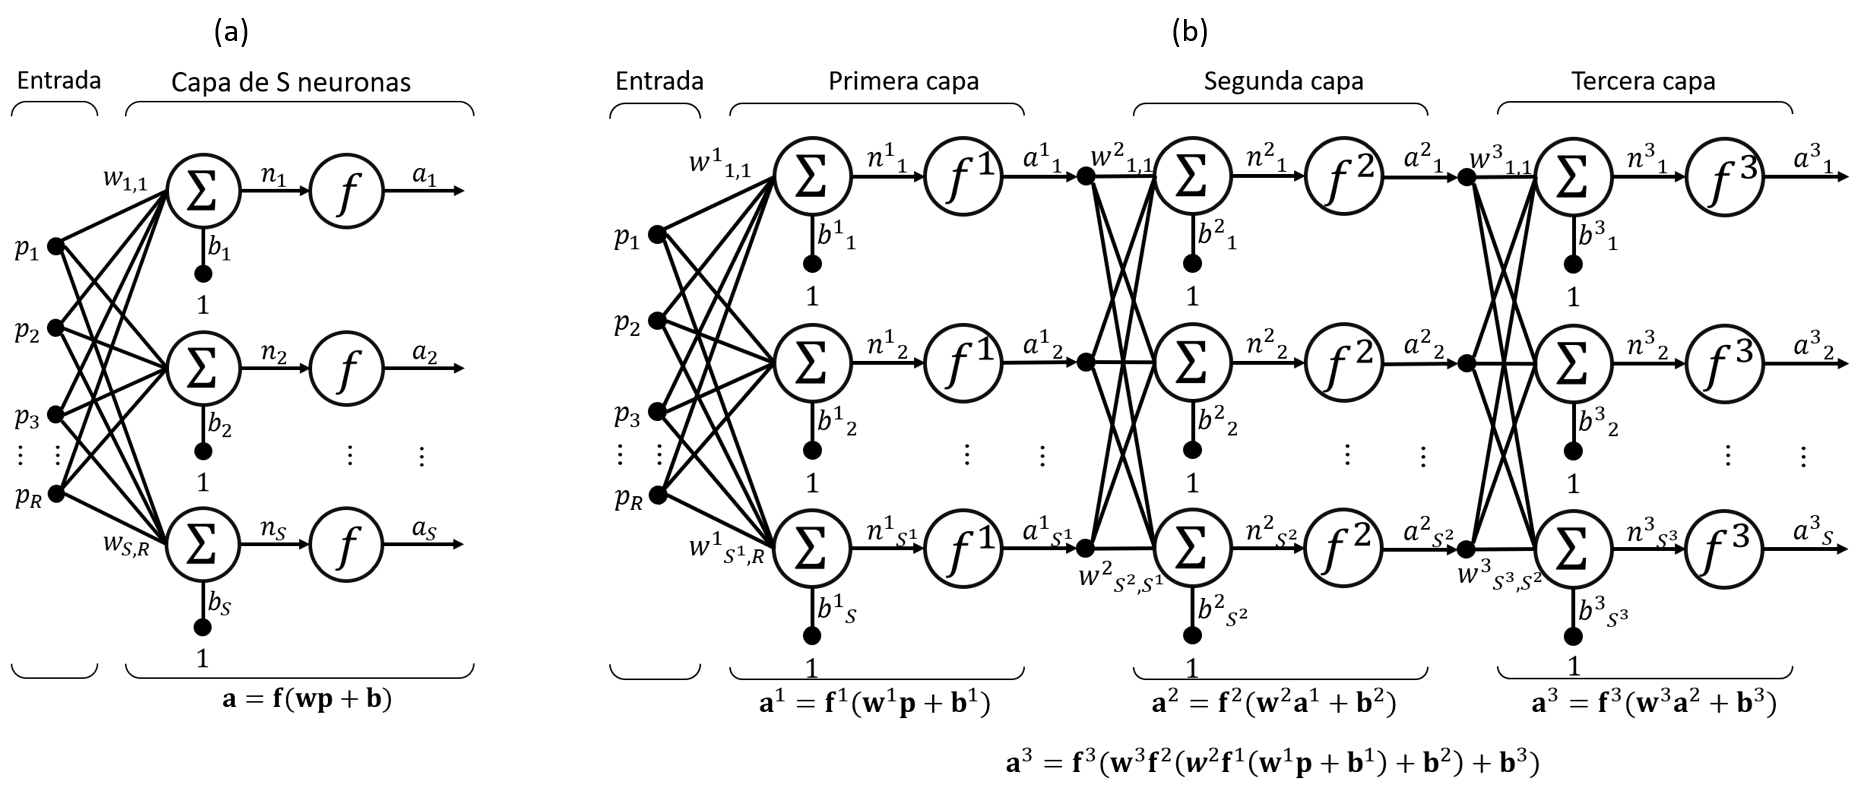
\includegraphics[width=.9\textwidth]{Imagenes/ConjuntoANN.png}
     \caption{Redes neuronales artificiales: (a) de capa oculta y (b) múltiples capas.}
    \label{fig:Net_conjunt}
 \end{figure}


El perceptron es conocido por ser el primer modelo de red neuronal, utilizado en clasificación de patrones a partir de entradas escalares binarias o vectores bipolares \citep{rosenblatt1958perceptron}. El algoritmo de aprendizaje se basa en la regla de Hebb, usando conjunto de datos de entrenamiento  para obtener los pesos de la red a través de iteraciones inicialmente con valores aleatorios.

\subsubsection{Funciones de activación}

Las funciones de activación es una función matemática que determina la salida de una neurona artificial en función de su entrada. Esta función introduce no linealidad en el modelo, lo que permite a las redes neuronales aprender y modelar relaciones complejas entre los datos de entrada y salida \citep{dubey2022activation}. Las funciones desempeñan un papel muy crucial en las redes neuronales al aprender características abstractas a través de transformaciones no lineales. Algunas de sus propiedades comunes son las siguientes: a) Debe agregar la curvatura no lineal en el panorama de optimización para mejorar la convergencia del entrenamiento de la red, b) No debería aumentar significativamente la complejidad computacional, c) No debería obstaculizar el flujo del gradiente durante el entrenamiento y d) debería conservar la distribución de datos para facilitar una mejor capacitación de la red.

Existen diferentes tipos de funciones de activación, cada una con sus propias características y aplicaciones. Entre las más comunes se encuentran las siguientes:

\begin{itemize}
    \item Función tipo escalón: Esta función es la más simple y toma un valor de 1 si la entrada es mayor o igual que un umbral determinado, y 0 en caso contrario.
    \item Función Sigmoide: Esta función toma un valor entre 0 y 1, asemejándose a una curva en forma de S.
    \item Función tangente hiperbólica: Esta función es similar a la función sigmoide, pero toma valor entre -1 y 1.
    \item Función ReLU (Unidad Lineal Rectificada): Esta función toma un valor igual a la entrada si esta es mayor o igual que cero, y 0 en caso contrario.
    \item Función Leaky ReLU: Esta función es similar a la función ReLU, pero introduce una pequeña pendiente negativa.
\end{itemize}

\subsection{Inteligencia artificial}

La inteligencia artificial (IA) es un campo de la ciencia de la computación, que se enfoca en crear máquinas inteligentes que puedan razonar, aprender y actuar de manera autónoma \citep{rouhiainen2018inteligencia}.

Las tecnologías basadas en IA es usada para mejorar y disfrutar una mayor eficiencia en distintos ámbitos de la vida. La aplicación se puede realizar en diversas situaciones y algunas de las más importantes son las siguientes:

\begin{itemize}
    \item Reconocimiento de imágenes estáticas, clasificación y etiquetado.
    \item Mejoras del desempeño de la estrategia algorítmica comercial.
    \item Procesamiento eficiente y escalable de datos de pacientes.
    \item Mantenimiento predictivo.
    \item Detección y clasificación de objetos
    \item Protección contra amenazas de cibernética.
\end{itemize}

Dentro de la IA se encuentran diversas técnicas para crear sistemas inteligentes, como el aprendizaje automático y aprendizaje profundo que son subcampos que desempeñan un papel fundamental en el análisis de grandes cantidades de datos, identificar patrones y tendencias, de una forma más rápida y precisa (Figura~\ref{fig:IA_AA_A}).

  \begin{figure}[!h]
     \centering
     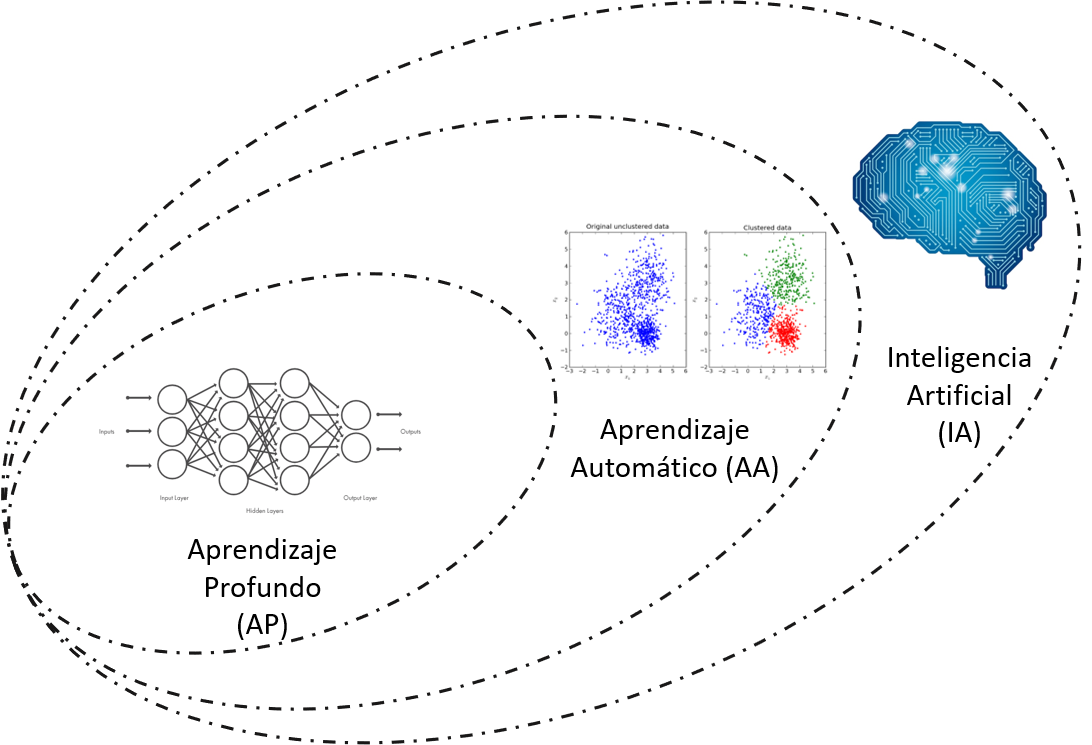
\includegraphics[width=.5\textwidth]{Imagenes/IA_AA_AP.png}
     \caption{Subcampos de la inteligencia artificial en el análisis de datos.}
     \label{fig:IA_AA_A}
 \end{figure}


\subsubsection{Aprendizaje Automático}

El aprendizaje automático (en inglés, \textit{machine learning}) se centra en el desarrollo de sistemas capaces de aprender de conjuntos de datos sin ser programados de manera explícita \citep{mitchell1997does}. Estos sistemas aprenden y mejoran su rendimiento en una tarea especifica a medida que se le presentan más datos. Un resultado típico serían las sugerencias o predicciones en una situación particular \citep{vieira2020main}.

Desde el punto de vista de ingeniería se define como un programa de computador que aprende de una experiencia E, con respecto a una tarea T y una medida de rendimiento R, si su rendimiento en T, medido por R, mejora con la experiencia E y también se puede definir como la ciencia de programar computadores para que aprendan a partir de un conjunto de datos \citep{geron2020aprende}.

\subsubsection{Aprendizaje Profundo}

El aprendizaje profundo (en inglés, \textit{deep learning}) es una rama del aprendizaje automático. A diferencia de los algoritmos tradicionales de aprendizaje automático, muchos de los cuales tienen una capacidad finita de aprendizaje independientemente de cuántos datos adquieran, los sistemas de aprendizaje profundo pueden mejorar su rendimiento al poder acceder a un mayor número de datos, o lo que es lo mismo, hacer que la máquina tenga más experiencia \citep{shinde2018review}. Una vez que las máquinas han conseguido suficiente experiencia mediante el aprendizaje profundo, pueden ponerse a trabajar para realizar tareas específicas como conducir un coche, detectar hierbajos en un campo de cultivo, detectar enfermedades, inspeccionar maquinaria para identificar errores, etc.

El aprendizaje profundo toma los fundamentos teóricos de las ANN clásicas, pero emplea una gran cantidad de neuronas y capas ocultas, junto con nuevos modelos y paradigmas de entrenamiento ofreciendo una capacidad mucho mayor para aprender a adaptarse y extraer características de datos de entrada de alta complejidad \citep{schmidhuber2015deep}. Las ANN usadas en el aprendizaje profundo son conocidas como redes neuronales profundas, en inglés \textit{Deep Neuronal Network} (DNN).

\subsection{Red Neuronal Convolucional}

Las redes neuronales convolucionales, en inglés, \textit{Convolutional Neuronal Network} (CNN) son un tipo algoritmo propuesto por LeCun en 1989 \citep{lecun1989backpropagation}. La aplicación de las CNN se encuentra principalmente en el reconocimiento de voz, reconocimiento facial, reconocimiento de objetos, análisis de movimiento y procesamiento de lenguaje natural.

Las CNN habitualmente constan de múltiples capas de convolución acompañadas de capas de agrupación y una capa de neuronas completamente conectadas, como se muestra en la Figura~\ref{fig:CNN}.

  \begin{figure}[!h]
     \centering
     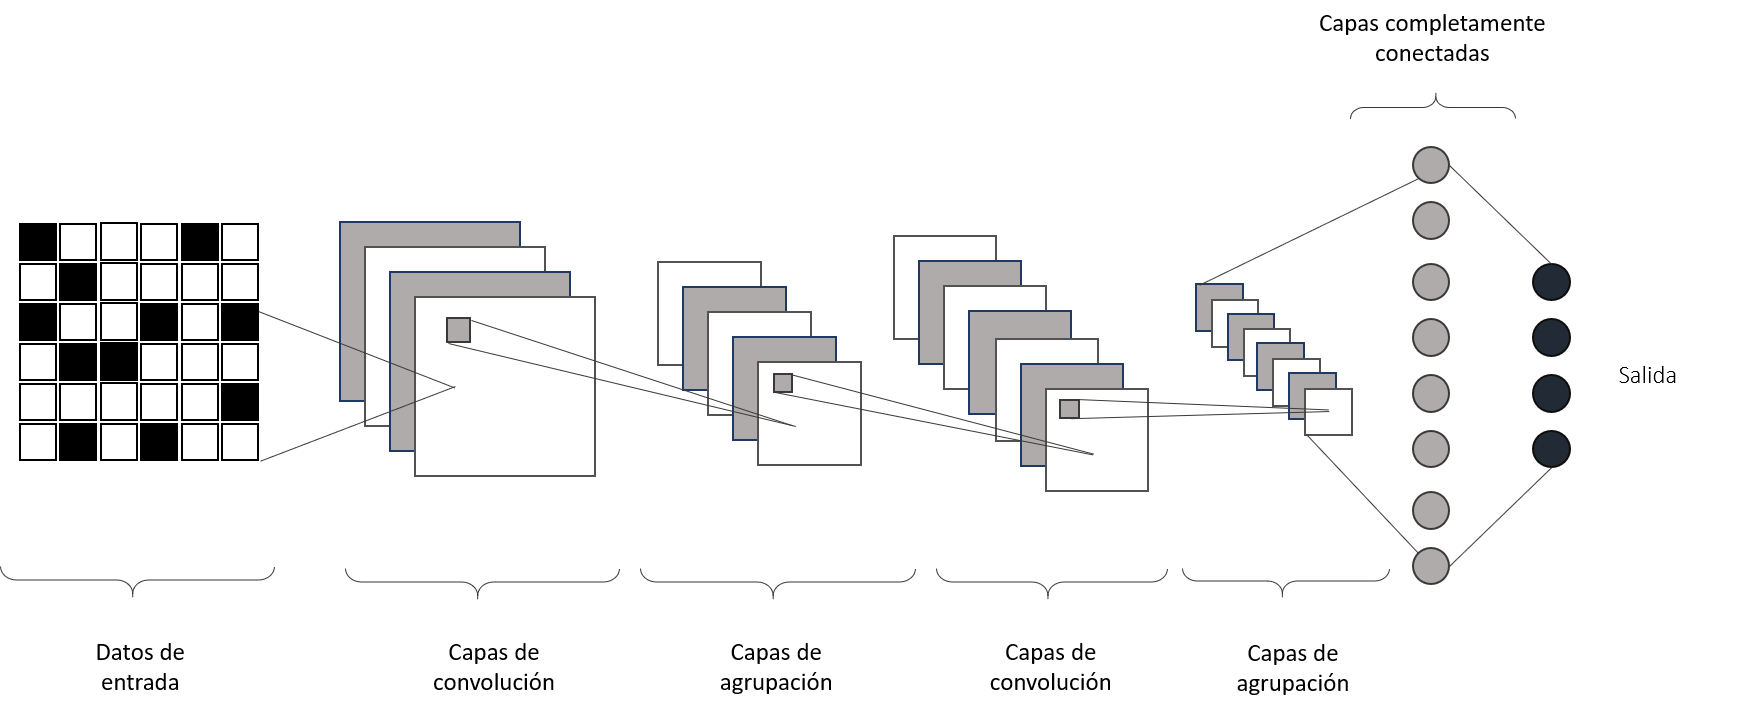
\includegraphics[width=.9\textwidth]{Imagenes/CNN.png}
     \caption{Diagrama de red convolucional simple.}
     \label{fig:CNN}
 \end{figure}

 La función de convolución se utiliza principalmente para extraer diversas características de los datos analizados. En proceso de la convolución cuenta de un núcleo de convolución, el cual se va deslizando en la ventana de entrada, de modo que los parámetros de peso en el núcleo se vayan multiplicando por los píxeles correspondientes. Posteriormente, los resultados siguen la multiplicación. En la Figura~\ref{fig:Convolution} se muestra el principio de la convolución.

 \begin{figure}[!h]
     \centering
     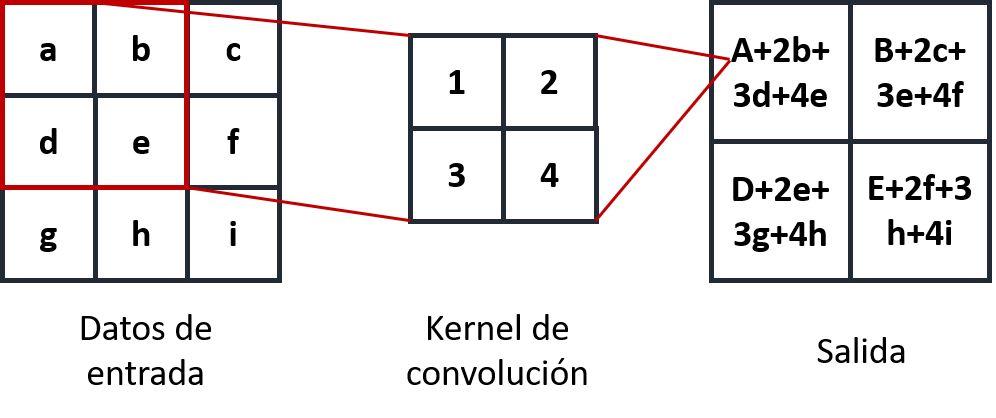
\includegraphics[width=.5\textwidth]{Imagenes/Convolucion.png}
     \caption{Diagrama esquemático de operación de convolucion.}
     \label{fig:Convolution}
 \end{figure}

 La función de la capa de agrupación es abstraer la señal característica original, lo cual se realiza para reducir en gran medida los parámetros de entrenamiento y también poder reducir el grado de sobreajuste. Las operaciones de agrupación se dividen en dos categorías: agrupación máxima y agrupación media. En la agrupación máxima se toma el valor más grande de un pixel correspondiente como resultado del muestreo, y en la agrupación media se calcula el valor promedio del pixel correspondiente. En la Figura~\ref{fig:Agrupacion} se muestra el principio de la agrupación.

  \begin{figure}[!h]
     \centering
     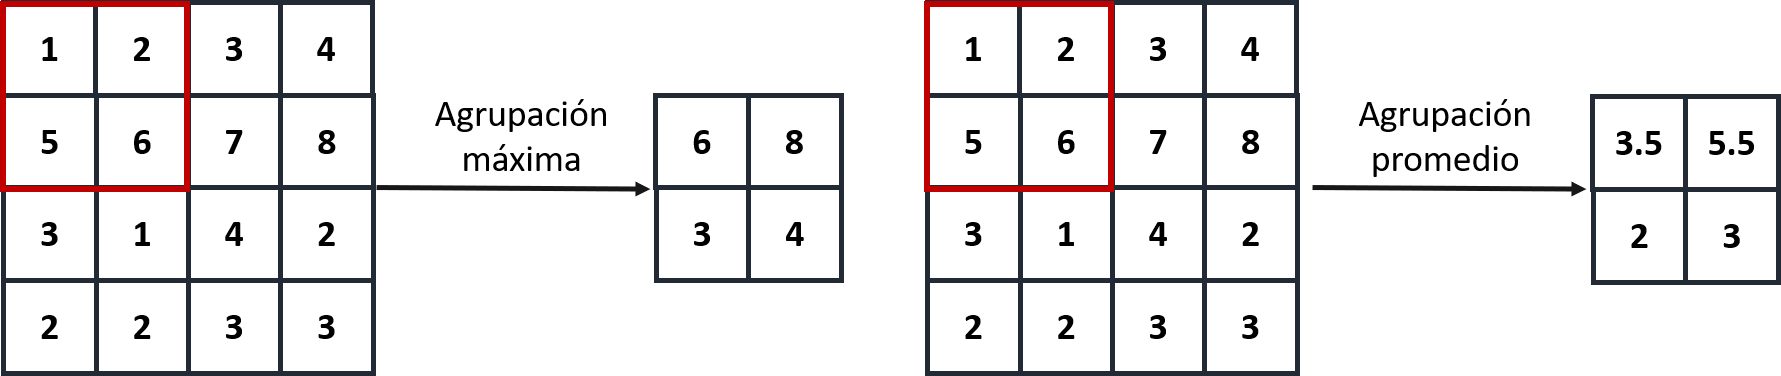
\includegraphics[width=.7\textwidth]{Imagenes/Agrupamiento.png}
     \caption{Diagrama esquemático de la operación de agrupación.}
     \label{fig:Agrupacion}
 \end{figure}

 \subsection{Red Neuronal Recurrente}

 Las redes neuronales recurrentes, en inglés, \textit{Recurrent Neuronal Network} (RNN) es un tipo de algoritmo propuesto en 1980. En los últimos años, las aplicaciones de las RNN han sido en muchos campos como: el procesamiento del lenguaje natural, el reconocimiento de imágenes y reconocimiento de voz.

 La característica principal de las RNN es que la entrada de la capa oculta incluye no solo la salida de capa de entrada, sino también la salida de la capa oculta en el último momento. Un modelo RNN simple puede ser expandido a una red compleja. En la Figura~\ref{fig:RNN} se puede observar la estructura de una RNN y el mapa de dependencia del orden temporal.

   \begin{figure}[!h]
     \centering
     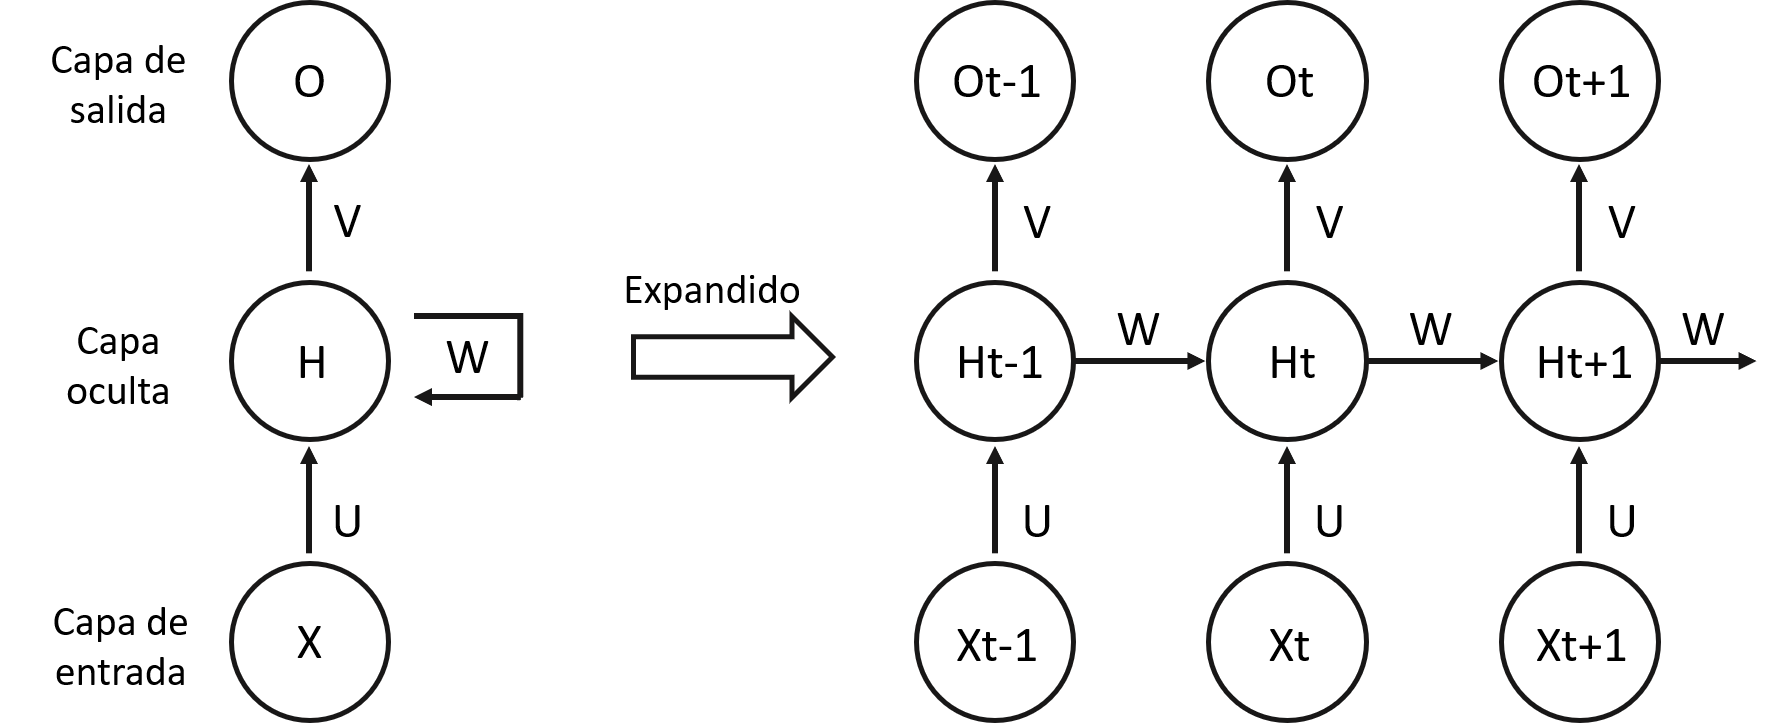
\includegraphics[width=.7\textwidth]{Imagenes/RNN.png}
     \caption{Estructura de la red neuronal recurrente simple y expandida.}
     \label{fig:RNN}
 \end{figure}

En la estructura de la RNN, Ht es el estado oculto del tiempo t y Ot representa la salida del tiempo t; U es el peso directo de la capa de entrada a la capa oculta; W es el peso de la capa oculta a la capa oculta, que es el controlador de memoria de la red que se encarga de programar la memoria; V es el peso de la capa oculta a la capa de salida, y las características aprendidas de la capa oculta pasaran a través de ella nuevamente y como salida final.
\section{Estado del arte}


Como ya se mencionó en la introducción, los datos ómicos abarcan diferentes conjuntos de datos que miden aspectos biológicos desde el ADN, el ARN, proteínas y metabolitos, en los últimos años se han desarrollado herramientas como la creación de bases de datos públicas para facilitar a los investigadores el acceso al análisis de estos datos y el desarrollo de métodos enfocados en la identificación, integración de datos y predicción.

El aprendizaje profundo ha revolucionado el análisis de datos ómicos, obteniendo información compleja y más precisa de conjuntos masivos de datos. Algunas de las principales aplicaciones en la biomedicina son el descubrimiento de biomarcadores, predicción de fenotipos, integración de datos ómicos, diseño de fármacos y regulación genética.

Se destacan algunas estructuras de ANN frecuentemente usadas en el análisis de datos ómicos como las redes neuronales convolucionales en la identificación de patrones espaciales, las redes neuronales recurrentes para modelar secuencias temporales, auto codificadores, redes neuronales profundas, redes generativas y codificadores automáticos variacionales.

Los principales desafíos que se presentan son que se requieren grandes conjuntos de datos para entrenamiento y su procesamiento es una tarea que compromete la eficiencia de la red, sesgo de los datos y la codificación de los datos.

En las siguientes secciones se abordará con más detalle sobre el estado del arte de los datos omicos, aprendizaje profundo y sus aplicaciones en el análisis de datos ómicos.

\subsection{Datos ómicos}

Las ciencias ómicas se refieren a la evaluación integral o global de una colección de características de un ser vivo, el estudio de genes y proteínas han identificado con éxito, características clave que influyen en la salud y la enfermedad. Los datos omicos han sido impulsados, debido al desarrollo y disponibilidad de tecnologías de matrices, espectrometría de masas de alto rendimiento y plataformas de secuenciación \citep{hasin2017multi}.

Los sistemas biológicos dependen de la transferencia de información de los ácidos nucleicos a las proteínas y metabolitos para dar forma a la función y fenotipo, es por esto que el estudio de las enfermedades es el resultado de procesos complejos y heterogéneos \citep{kim2018data}. Los datos omicos son utilizados para el análisis de valores atípicos en una secuencia, lo cual puede indicar la progresión de una enfermedad y permite aprovecharse como indicadores para un diagnóstico temprano, con esto se pueden perfeccionar los enfoques de detección y diagnóstico, así como también identificar y personalizar intervenciones o tratamientos \citep{krassowski2020state}.

Dentro de las ciencias ómicas frecuentemente utilizadas se encuentran: la genómica, transcriptómica, proteómica y la epigenómica, a continuación se detalla un poco más sobre estas ciencias:

La genómica se encarga de la caracterización del contenido genético de un organismo, típicamente consiste en ADN (ARN en algunos virus), la secuenciación del genoma es utilizada para identificación de nuevos genes y variantes genéticas y mediante estudios de asociación de todo el genoma se relacionan variantes genómicas con estados patológicos u otros fenotipos.

La transcriptómica se centra en el estudio del ARN codificante de proteínas (ARN mensajero), las señales transcriptómicas proporcionan información sobre los genes y mecanismos potenciales implicados en un proceso biológico de interés.

La proteómica estudia las proteínas expresadas, las moléculas fundamentales para la vida y su funcionamiento en los organismos vivos. Esta información tiene el potencial para mejorar la compresión de la biología, el diagnóstico de enfermedades y desarrollo de tratamientos.

La epigenómica aborda la caracterización de todo el genoma, de modificaciones químicas reversibles del ADN o de proteínas asociadas al ADN que afectan la expresión y regulación de genes. Las modificaciones epigenómicas pueden proporcionar información sobre el estado de la enfermedad y/o la exposición ambiental y actuar como rasgos hereditarios.

Uno de los aspectos actuales más destacados en la investigación omica es la integración de datos ómicos (multiómica) de diferentes niveles moleculares con el fin de obtener una visión holística de los sistemas biológicos. Se han encontrado desafíos en la integración de datos como la heterogeneidad de datos, la fata de estándares de datos y la complejidad computacional.

\subsubsection{Análisis de datos omicos}

La tecnología de análisis de datos omicos ha cambiado la forma en la que se estudian las enfermedades, permitiendo conocer los cambios a nivel molecular que intervienen en diversos padecimientos. A través de los datos omicos se obtiene una compresión de las causas y mecanismos de las enfermedades, con lo cual se abren oportunidades en aplicaciones de diagnóstico, tratamiento y prevención por medio del descubrimiento de nuevos biomarcadores biológicos \citep{reel2021using}.

Un biomarcador es una sustancia, estructura o proceso que se puede medir en el cuerpo humano o sus productos y puede proporcionar información importante sobre la presencia de una enfermedad o afección \citep{strimbu2010biomarkers}. Los biomarcadores moleculares se descubren analizando grandes cantidades de información proporcionada de diferentes ómicas y estos desempeñan un papel importante en la planificación de medidas y decisiones preventivas para los pacientes en el diagnóstico, pronóstico o predicción. Los biomarcadores de diagnóstico se utilizan para determinar la presencia de una enfermedad en un paciente, por otro lado, los biomarcadores de pronóstico brindan información sobre el resultado general con o sin tratamiento. Los biomarcadores predictivos se utilizan para identificar el riesgo de sufrir algún resultado \citep{carlomagno2017diagnostic}.

Dentro de las principales enfermedades analizadas en omica e identificación de biomarcadores se encuentran:

El cáncer debido a que es una de las principales causas de muerte en el mundo y la omica ha contribuido significativamente a la compresión de su complejidad \citep{sarmiento2020aplicaciones}. En el diagnóstico, el análisis ómico ha permitido la identificación de biomarcadores moleculares para la detección de cáncer en una etapa temprana, incluso antes de la presencia de síntomas. En el pronóstico se puede predecir el curso de la enfermedad y la probabilidad de respuesta al tratamiento, la expresión genética de ciertos genes puede usarse para predecir el riesgo de recurrencia del cáncer. En el tratamiento se han impulsado el desarrollo de terapias dirigidas, que se enfocan en las mutaciones genéticas especificas que impulsan el crecimiento del cáncer. Y en la prevención se usa para la identificación de individuos con un alto riesgo de desarrollar cáncer, lo que permite implementar estrategias de prevención personalizar\citep{munir2019cancer}.

Las enfermedades cardiovasculares, como los ataques cardiacos y los accidentes cerebrovasculares, son otra de las causas de muerte a nivel global. En el diagnóstico se puede predecir el riesgo de presentar enfermedades cardiovasculares en el que se analizan los niveles de lipoproteina de baja densidad y de alta densidad que se asocian a un mayor riesgo de enfermedad cardiaca. En el tratamiento, la omica ha contribuido en el desarrollo de fármacos para implementación en pacientes con dicha patología \citep{pasha2020cardiovascular}. En la prevención se utiliza para identificar en una persona propensa a desarrollar enfermedades cardiovasculares, lo cual permite implementar estrategias de prevención personalizada, como cambios en estilo de vida, dieta saludable y actividad física para reducir el riesgo en individuos con predisposición genética \citep{wang2017detecting}.

Las enfermedades neurodegenerativas, como el Alzheimer y el Parkinson, son un grupo de enfermedades progresivas que afectan el sistema nervioso central y provocan una perdida progresiva de la función cerebral. La omica en el diagnóstico permite identificar biomarcadores asociados con estas enfermedades, el pronóstico permite conocer la progresión de la enfermedad y predecir la tasa de deterioro cognitivo, en el tratamiento permite el desarrollo de fármacos que permitan tratar estas enfermedades y la prevención para identificar individuos con un alto riesgo de desarrollo de este tipo de enfermedades, lo que permite implementar estrategias de prevención personalizadas \citep{erdacs2021neurodegenerative}.

Enfermedades infecciones, normalmente causadas por patógenos como virus, bacterias y parásitos, que es un problema de salud publica recurrente e importante, la omica en el diagnóstico permite identificar los biomarcadores por medio de detección genética viral, en el tratamiento de para desarrollo de nuevos antibióticos y antivirales más efectivos y en la prevención para identificar a las personas más propensas a desarrollar enfermedades infecciones e implementar estrategias como las vacunas \citep{chae2018predicting}.



\subsubsection{Bases de datos ómicos}

La producción de datos omicos incrementa cada año. es por esto que se han establecido diversas bases de datos bioinformáticas que contienen diferentes tipos de datos moleculares, como secuencias de ADN, perfiles de expresión genética, datos de metilación de ADN y variantes genéticas. La adquisición de datos para entrenamiento y validación de los modelos de aprendizaje profundo ya no se considera un problema, en la Tabla \ref{tab:bases_de_datos} siguiente se presentan varias bases de datos de uso común en la rama ómica \citep{zhang2019deep}.

\begin{table}[h!]
    \scriptsize
    \centering
    \caption{Bases de datos ómicos disponibles de libre acceso}
    
    \begin{tabular}{
    >{\centering\arraybackslash}m{6cm} 
    >{\centering\arraybackslash}m{3cm}}
\hline 
        \textbf{Enfoque de la base de datos} & 
        \textbf{Nombre}
\\      
    \hline \hline 

     Datos de genoma &
    {\href{https://www.ncbi.nlm.nih.gov/genome}{NCBI}}
    \\
    &
     {\href{https://www.ensembl.org/index.html}{Ensembl}}
     \\
      &
      {\href{https://www.ensembl.org/index.html}{UCSC}}
     \\
\hline
      Secuenciación de genoma de tipos de cáncer &
     {\href{https://portal.gdc.cancer.gov/}{TCGA}}
    \\
    \\
\hline
      Secuencias de ácidos nucleicos
     &
     {\href{https://www.ebi.ac.uk/ena/browser/home}{ENA}}
     \\
     &
     {\href{https://www.ncbi.nlm.nih.gov/genbank/}{GenBank}} 
     \\
     &
     {\href{https://www.ddbj.nig.ac.jp/index-e.html}{DDBJ}}
     \\
\hline
     Secuencias de proteínas &
     {\href{https://www.uniprot.org/uniprotkb/P51587/entry}{Swiss-prot}}
\\ 
%----------------------------------------------------------
     &
     {\href{https://proteininformationresource.org/}{PIRR}}
     \\
\hline 
     Estructura proteínicas
     &
     {\href{https://www.rcsb.org/pdb}{PDB}}
     \\
\hline     
     Clasificación de estructuras proteínicas &
     {\href{https://scop.berkeley.edu/}{SCOPe}}
     \\
     &
{\href{http://www.cathdb.info/}{CATH}}
     \\
    \hline 
    \end{tabular}
    \label{tab:bases_de_datos}
\end{table}

Este tipo de datos comúnmente tienen formatos del tipo fasta, fastaq, gff2, bed, etc. Propios de su estándar industrial, para aplicación de aprendizaje profundo puede ser necesario conocer lenguajes de programación como Perl, R o Python para la extracción de información y posteriormente ordenar los datos en una forma que los modelos de aprendizaje profundo puedan interpretar como matrices y vectores.

Actualmente, existe una gran cantidad de datos omicos para diversas aplicaciones en la investigación médica actual impulsadas por tecnología de secuenciación de los cuales destaca la investigación del cáncer que es uno de los mayores proveedores de datos omicos moleculares a gran escala, que proporciona soporte de datos integral desde la perspectiva de diferentes procesos biológicos y ayuda a explorar la patogénesis de todo tipo de cáncer y tumores cancerígenos \citep{li2024avbae}.

\subsection{Aprendizaje profundo}

El aprendizaje profundo es un campo de la inteligencia artificial, se ha impulsado debido a la disponibilidad de conjuntos de datos, recursos computacionales y algoritmos innovadores. El campo de aplicación es amplio, pero se tienen investigación importante recientes como:

\begin{itemize}

   \addtolength{\itemsep}{-4mm} %con esto se ajusta el interlineado entre la lista
        \item En la ciencia para análisis de conjunto de datos científicos y realizar descubrimientos en las áreas de la física, química y biología.

        \item DL aplicado en atención médica, desarrollando herramientas de diagnóstico y tratamiento para enfermedades como el cáncer, enfermedades cardiacas y enfermedades neurológicas.

    \end{itemize}

\subsubsection{Aprendizaje profundo en ómica}

El DL en el área de la genómica se ha usado para predecir las unidades funcionales de las secuencias de ADN, predecir el dominio de replicación, predicción del factor de transcripción, el punto de iniciación de la transcripción, el promotor, el potenciador y el sitio de borrado del gen \citep{quang2019factornet,umarov2017recognition,zeng2016convolutional,zhang2017titer,min2017predicting,singh2019predicting,lee2015dna}. En los últimos años, se ha impulsado el uso de redes neuronales convolucionales enfocado en la predicción de promotores, potenciadores, dominios de replicación, detección de supresiones genéticas y diferenciación de exones de intrones. El uso de Redes Neuronales Convolucionales (CNN) se ha impulsado en los últimos años en la predicción de promotores, potenciadores, dominio de replicación, detección de supresiones genéticas y diferenciación de exones de intrones.

También se destaca el uso de aprendizaje profundo para predicción de la expresión genética. Esto implica en la predicción del gen objetivo, de la función génica, modelado de redes de regulación génica, etc. En estas aplicaciones, los datos de entrenamiento utilizados frecuentemente son: secuencias de ADN y datos de modificación de histonas. Las redes neuronales especializadas para esta aplicación son las CNN y las RNN \citep{quang2016danq,raza2016recurrent,zhou2015predicting,cuperus2017deep,koh2017denoising}.

Se encuentran trabajos importantes del uso de aprendizaje profundo para explorar genomas y enfermedades epigenéticas y otros campos. Los datos de entrenamiento frecuentemente usados son: el mapa genómico, los perfiles de expresión genética y datos clínicos. En este campo de aplicación los esquemas de redes neuronales es más amplió como CNN, RNN, Auto-codificadores, Redes Generativas \citep{liang2014integrative,yousefi2017predicting,young2017unsupervised}.

El DL en la transcriptómica se analiza la estructura de secuencias de ARN como los sitios de unión de RBP, sitios de empalme alternativo y los tipos de ARN. Para el entrenamiento, los datos frecuentemente utilizados son las secuencias de ARN, estructuras secundarias y terciarias de ARN y CLIP-seq. En estas aplicaciones las redes CNN y RNN son las ma utilizadas \citep{xu2017deep,zhang2017sequence,pan2017rna}.

Las aplicaciones más relevantes es la asociación entre el ARN y las enfermedades o entre el ARN y el diseño de fármacos. Para el entrenamiento de DL se utilizan datos de secuencias de ARN (miRNA-seq), transcriptómica en el mapa genético y datos metilación de ARN. Para estas aplicaciones el uso de esquemas de redes neuronales es más amplio como CNN, RNN, AE y GAN \citep{chaudhary2018deep,yu2018drug,aliper2016deep,bhat2016deepcancer}.

El DL en proteómica se usa en la identificación de estructura de proteínas, como la predicción de la estructura terciaria y secundaria de proteínas, evaluación del modelo de proteínas, predicción del mapa de contacto de proteínas, etc. Los datos que se utilizan en el entrenamiento son la secuencias de aminoácidos, estructuras bidimensionales de proteínas y propiedades fisicoquímicas de aminoácidos. En esta aplicación se encuentran las redes neuronales profundas (DNN) con un cambio al uso de RNN \citep{stahl2017epsilon,li2017deep,spencer2014deep,heffernan2015improving}.

También se destaca el uso de DL en la predicción de la función de proteínas, donde los datos utilizados para el entrenamiento del modelo son secuencias de aminoácidos, la estructura de la proteína e interacciones proteína-proteína, el tipo de redes más usadas son las CNN y las RNN \citep{kulmanov2018deepgo,wang2017musitedeep}.

En la siguiente Tabla~\ref{tab:revision} se muestra la revisión de los algoritmos de aprendizaje profundo utilizados para propósitos de clasificación, predicción, codificación de los datos, y el tipo de datos utilizados.

\begin{table}[!h]
    \scriptsize
    \centering
    \caption{Revisión del estado del arte de algoritmos utilizados en clasificación, identificación, codificación y clasificación}
    
    \begin{tabular}{
    >{\centering\arraybackslash}m{2cm} 
    >{\centering\arraybackslash}m{2cm}
    >{\centering\arraybackslash}m{1.2cm} 
    >{\centering\arraybackslash}m{1.25cm}
    >{\centering\arraybackslash}m{1.2cm} 
    >{\centering\arraybackslash}m{2cm}
    >{\centering\arraybackslash}m{1.4cm} 
    >{\centering\arraybackslash}m{1.6cm}
    >{\centering\arraybackslash}m{1.5cm}}
\hline 
        \textbf{\tiny{Algoritmo de DL}} & 
        \textbf{\tiny{Tipo de datos omicos}} &
        \textbf{\tiny{Predicción}}  &
        \textbf{\tiny{Clasificación}}  &
        \textbf{\tiny{Codificación}}  &
        \textbf{\tiny{Preprocesamiento}}  &
        \textbf{\tiny{Entrenamiento y validación}}  &
        \textbf{\tiny{Propósito}}  &
        \textbf{\tiny{Referencia}}
\\      
    \hline \hline 

    \tiny{MLP (perceptron multicapa), CNN} &
    \tiny{Transcriptómico, Metabolómicos} &
    x &
    x &
    x &
    x &
    &
    \tiny{Clasificación de etapas de cáncer} &
    \tiny{\citep{yu2019architectures}}
\\ 
    \tiny{XomiVAE} &
    \tiny{Genomico} &
     &
    x &
    x &
    x &
    x &
    \tiny{Clasificación de tipo de tumores} &
    \tiny{\citep{withnell2021xomivae}}
\\ 
    \tiny{Auto Encoder} &
    \tiny{Genómico, transcriptomico} &
     &
    x &
    x &
    x &
    x &
    \tiny{Clasificación de tipos de cancer} &
    \tiny{\citep{franco2021performance}}
\\ 
    \tiny{Deep Prog (CNN y ML)} &
    \tiny{Genómico, transcriptomico} &
    x &
    x &
    x &
    x &
    x &
    \tiny{Clasificación de tipos de cancer} &
    \tiny{\citep{poirion2021deepprog}}
\\
    \tiny{FactorNet (CNN)} &
    \tiny{Genómico, transcriptomico} &
    x &
     &
     &
    x &
    x &
    \tiny{Predicción de factores de transcripción} &
    \tiny{\citep{quang2019factornet}}
\\
    \tiny{CNN, AE, RNN} &
    \tiny{Genómico, epigenómico} &
    x &
     &
     &
    x &
    x &
    \tiny{Predicción metástasis cáncer} &
    \tiny{\citep{albaradei2021machine}}
\\
    \tiny{DCAP} &
    \tiny{Genómico, epigenomico} &
    x &
     &
    x &
    x &
    x &
    \tiny{Predicción tipos cáncer} &
    \tiny{\citep{chai2021integrating}}
\\
    \tiny{VAE} &
    \tiny{Genómico, transcriptomico} &
     &
    x &
     &
    x &
    x &
    \tiny{Clasificación de tipos de cáncer} &
    \tiny{\citep{leng2022benchmark}}
\\
    \tiny{AE, VAE, GAN} &
    \tiny{Genómico, epigenómico} &
    x &
     &
    x &
    x &
    x &
    \tiny{Imputacion de datos faltantes} &
    \tiny{\citep{huang2023deep}}
\\
    \tiny{CNN} &
    \tiny{Genómico, transcriptómico, proteómico} &
    x &
    x &
    x &
    x &
    x &
    \tiny{Identificacion de cancer y clasificacion} &
    \tiny{\citep{chuang2021convolutional}}
\\
    \tiny{DCNN} &
    \tiny{Genómico, transcriptómico} &
    x &
    x &
     &
    x &
    x &
    \tiny{Identificación de cáncer y clasificación} &
    \tiny{\citep{ma2018omicsmapnet}}
\\
    \tiny{DNN, CNN} &
    \tiny{Genómico, transcriptómico} &
    x &
     &
     &
     &
     &
    \tiny{Predicción de expresión genética} &
    \tiny{\citep{talukder2021interpretation}}
\\
    \tiny{CNN} &
    \tiny{Genómico} &
    x &
     &
    x &
    x &
     &
    \tiny{Prediccion de variantes no codificantes} &
    \tiny{\citep{eraslan2019deep}}
\\
    \tiny{CNN, RNN, AE, GAN} &
    \tiny{Genómico, transcriptómico} &
    x &
    x &
    x &
    x &
     &
    \tiny{Resolución unicelular} &
    \tiny{\citep{erfanian2023deep}}
\\
    \tiny{DeepMO} &
    \tiny{Genómico, transcriptómico} &
     &
    x &
    x &
    x &
    x &
    \tiny{Clasificación de cáncer} &
    \tiny{\citep{li2020deep}}
\\
    \tiny{MOADLN} &
    \tiny{Genómico, transcriptómico} &
    x &
    x &
     &
    x &
     &
    \tiny{Clasificación de subtipos de cáncer} &
    \tiny{\citep{gong2023multi}}
\\
    \tiny{CNN} &
    \tiny{Genómico, transcriptómico, epigenmico} &
    x &
    x &
    x &
    x &
    x &
    \tiny{Clasificación de cáncer} &
    \tiny{\citep{li2022machine}}
\\
    \tiny{DeepProg} &
    \tiny{Genómico, transcriptómico, epigenomico} &
    x &
    x &
    x &
    x &
     &
    \tiny{Diagnóstico de cáncer} &
    \tiny{\citep{mathema2023deep}}
\\
\hline
    \end{tabular}
    \label{tab:revision}
\end{table}

En la revisión anterior se puede observar que las principales aplicaciones de los datos omicos es enfocado en identificación y diagnóstico de cáncer debido es una de las enfermedades más importantes actualmente, por esto mismo se ha desarrollado una mayor cantidad de bases de datos. El tipo de algoritmos de aprendizaje profundo más utilizados son el CNN en aplicaciones de predicción y clasificación, seguido de las RNN.

\begin{table}[!h]
    \scriptsize
    \centering
    \caption{Bases de datos enfocadas en el análisis de datos omicos de tipos de cáncer.}
    
    \begin{tabular}{
    >{\centering\arraybackslash}m{2cm} 
    >{\centering\arraybackslash}m{3cm}
    >{\centering\arraybackslash}m{2cm} 
    >{\centering\arraybackslash}m{2cm}}
\hline 
    \textbf{Nombre de la base de datos} & 
    \textbf{Tipo de datos} &
    \textbf{Acceso a tipos de cáncer}  &
    \textbf{Formatos de descarga}
\\      
\hline \hline 

    TCGA &
    Genómica, transcriptómica, proteómica, metabolómica &
    33 tipos &
    JSON, TSV 
\\
    GEO &
    Genómica, transcriptómica, proteómica &
    20 tipos &
    JSON, TSV
\\  
    ICGC &
    Genómica, transcriptómica, proteómica, metabolómica &
    50 tipos &
    JSON, TSV 
\\
    CBioPortal &
    Genómica, transcriptómica, proteómica &
    200 tipos &
    JSON, TSV 
\\
    NCI &
    Genómica, transcriptómica, proteómica &
    30 tipos &
    JSON, TSV 
\\
    CBDiscovery &
    Genómica, transcriptómica, proteómica &
    25 tipos &
    JSON, TSV 
\\
\hline
    \end{tabular}
    \label{tab:base_datos_cancer}
\end{table}

El análisis de datos omicos actualmente se centra en el cáncer y, por lo tanto, se ubica un mayor número de bases de datos genómicos, transcriptómicos, proteómicos y metabolómicos. Esto presenta una ventaja debido a que se tiene un mayor número de datos de entrenamiento y validación para los investigadores que se dedican al desarrollo de algoritmos de aprendizaje profundo. En la Tabla~\ref{tab:base_datos_cancer} se muestran las distintas bases de datos de distintos tipos de cáncer, destacando la TCGA debido a cuenta con una biblioteca para la descarga por lotes de datos y que ha sido de mayor uso en los trabajos de investigación \citep{li2022identification}.


De esta revisión se logra precisar sobre el tipo de datos que se seleccionaran para el diseño del algoritmo de red neuronal, debido a que los datos enfocados en el cáncer cuentan con el mayor número de bases de datos del cual adquirir conjuntos de entrenamiento. En la Tabla~\ref{tab:RevisionCancer} se toman trabajos con este enfoque.

\begin{table}[!h]
    \scriptsize
    \centering
    \caption{Revision de articulos enfocados en cancer destacando conjunto de entrenamiento, tipos de datos y base de datos utlizada.}
    
    \begin{tabular}{
    >{\centering\arraybackslash}m{2cm} 
    >{\centering\arraybackslash}m{2cm}
    >{\centering\arraybackslash}m{2cm} 
    >{\centering\arraybackslash}m{2cm}
    >{\centering\arraybackslash}m{2cm}
    >{\centering\arraybackslash}m{1.5cm} 
    >{\centering\arraybackslash}m{2cm}}
\hline 
    \textbf{Proposito} & 
    \textbf{Conjuto de datos} &
    \textbf{Genomica}  &
    \textbf{Transcriptómica} &
    \textbf{Base de datos} & 
    \textbf{Otros} &
    \textbf{Referencia}
    
\\      
\hline \hline 

    Pronostico de supervivencia &
    15 tipos  &
    x &
    x &
    TCGA &
    &
    \citep{huang2023deep}
\\
\hline
\\
    Clasificación de cáncer &
    11 tipos &
     &
    x &
    TCGA &
    Datos clinicos&
    \citep{chuang2021convolutional}
\\
\hline
\\
    Clasificación de cáncer &
    33 tipos &
    x &
    x &
    TCGA &
    &
    \citep{franco2021performance}
\\
\hline
\\
    Predicción de supervivencia &
    32 conjuntos multiomicos &
    x &
    x &
    TCGA &
    &
    \citep{chuang2021convolutional}
\\
\hline
\\
    Clasificación de cáncer &
    33 tipos &
    x &
    x &
    TCGA &
    &
    \citep{withnell2021xomivae}
\\
\hline
\\
    Clasificación de cáncer y agrupamiento de cáncer&
    5 tipos &
    x &
    x &
    TCGA &
    &
    \citep{chuang2021convolutional}
\\
\hline
\\
    Clasificación de cáncer &
    33 tipos &
    x &
    x &
    TCGA &
    &
    \citep{zhang2019deep}
\\
\hline
\\
    Predicción de supervivencia &
    1 tipo &
    x &
    x &
    TCGA &
    &
    \citep{tong2020deep}
\\
\hline
    \end{tabular}
    \label{tab:RevisionCancer}
\end{table}


El creciente éxito de aprendizaje profundo ha impulsado el desarrollo de software de código abierto, en las que se encuentran las más populares como tensorflow, Caffe, Torch y CNTK. Estas herramientas son compatibles con CPU multinucleo y GPU multinucleo\citep{shi2016benchmarking,liu2020application}.

Tensorflow desarrollador por Google integra unidades más comunes en el marco del aprendizaje profundo. Soporta redes actualizadas como CNN y RNN con diferentes configuraciones. Este marco está diseñado para ofrecer flexibilidad, portabilidad y alta eficiencia del hardware equipado.

Caffe desarrollador por Berkeley Vision and Learning Center (BVLC) y es de código abierto desde 2014. Caffe puede procesar 40 millones de imágenes al día con la version acelerada por GPU en una sola tarjeta GPU NVIDIA k40 o Titan. Con integración cuDNN, se consigue otra aceleración 1.3k \citep{chetlur2014cudnn}.

CNTK es un conjunto de herramientas de redes computacionales unificadas desarrolladas por Microsoft Research, que admite muchas redes neuronales populares. Este marco con múltiples GPU cuenta con un rendimiento bastante aceptable comparándolo con otros\citep{huang2015microsoft}.

Torch es un marco de computación científica que proporciona estructuras de datos para los componentes más útiles en algoritmos de aprendizaje automático, como tensores multidimensionales y operaciones matemáticas sobre ellos.
%-----------------------------------------------



\section{Propuesta de tesis}

\subsection{Objetivo general}

\begin{itemize}

   \addtolength{\itemsep}{-4mm} %con esto se ajusta el interlineado entre la lista
        \item Modelar datos ómicos (genómicos, transcriptómicos y proteómicos) utilizando técnicas de aprendizaje profundo, empleando redes neuronales de diseño propio, y configurar la salida del modelo para diferentes propósitos de clasificación y predicción.

    \end{itemize}



\subsection{Objetivos específicos}

\begin{itemize}

   \addtolength{\itemsep}{-4mm} %con esto se ajusta el interlineado entre la lista
        \item Codificar datos genómicos, transcriptómicos y proteómicos para ser alimentados en las redes neuronales.
        \item Implementar redes neuronales convolucionada (CNN) y recurrente (RNN), y entrenarlas.
        \item Proponer y diseñar una red neuronal propia a partir de las dos anteriores.
        \item Configurar en cada caso la salida, si es un clasificador, un predictor, un regresor o un generador de señal.
        \item Enfocar el modelado de las redes neuronales para fines biomédicos.
        \item Validar los resultados con las bases de datos e incluyendo opinión de especialistas.
    \end{itemize}

\subsection{Antecedentes}

El aprendizaje profundo actualmente tiene como base de procesamiento a las redes neuronales, en CENIDET se cuentan con trabajos relacionados con la aplicación de algoritmos de redes neuronales artificiales.

Uno de los principales intereses es la participación con especialistas que participan en el área médica en el centro oncológico de San Peregrino Cancer Center, donde se tiene un convenio de participación. De misma manera se tiene una colaboración con la Universidad de Grenoble, donde se ha estado trabajando con datos omicos.

\subsection{Planteamiento del problema}

La conjunción del aprendizaje profundo en el área biomédica recientemente está dando resultados, como es una tecnología relativamente nueva, existen múltiples problemáticas por abordar como la alta dimensionalidad de datos, datos desequilibrados, explicabilidad de los modelos, estandarización de datos de las bases públicas, la imputación de datos y la clasificación errónea.

Las áreas de oportunidad que se plantean abordar son la codificación de datos en un formato que pueda ser interpretado y analizado por el modelo de red neuronal, donde se considera la normalización de los datos adquiridos, imputación y reducción de dimensiones con el fin de aumentar la precisión del modelo de DL.

Los algoritmos de aprendizaje profundo en aplicaciones de clasificación y predicción utilizando datos omicos están lejos de ser óptimos debido a la complejidad de los tipos de datos y los problemas antes mencionados, lo que se busca abordar es en la propuesta de un nuevo algoritmo que tome las ventajas que tienen otros e incorporarlas, ya que como se propone vincular con el área médica se requiere una alta precisión en las respuestas que se obtienen del modelo.

\subsection{Pregunta de investigación}

¿Es posible proponer un modelo de red neuronal basado en aprendizaje profundo que ayude a aumentar la precisión en la clasificación/predicción de un fenotipo utilizando datos genómicos, transcriptómicos y genómicos que pueda utilizarse en el área biomédica?

\subsection{Justificación}

El uso de datos omicos de diversas fuentes públicas presenta problemas como la heterogeneidad y datos desequilibrados (datos faltantes y/o mal etiquetados), con el uso de algoritmos de aprendizaje profundo enfocados en la imputación y codificación se podría mejorar la eficiencia de predicción y clasificación del modelo para pronóstico del cáncer. La integración con el área biomédica supone una ventaja en el área biomédica para una evaluación temprana en pacientes con un tipo de cáncer y determinar la progresión con el cual se pueden establecer tratamientos adecuados.
\section{Cronograma de actividades}

En esta sección se muestra es cronograma de las actividades que de manera preliminar se planean abordar los 4 años de estancia en CENIDET.

\begin{figure}[h!]
    \centering
    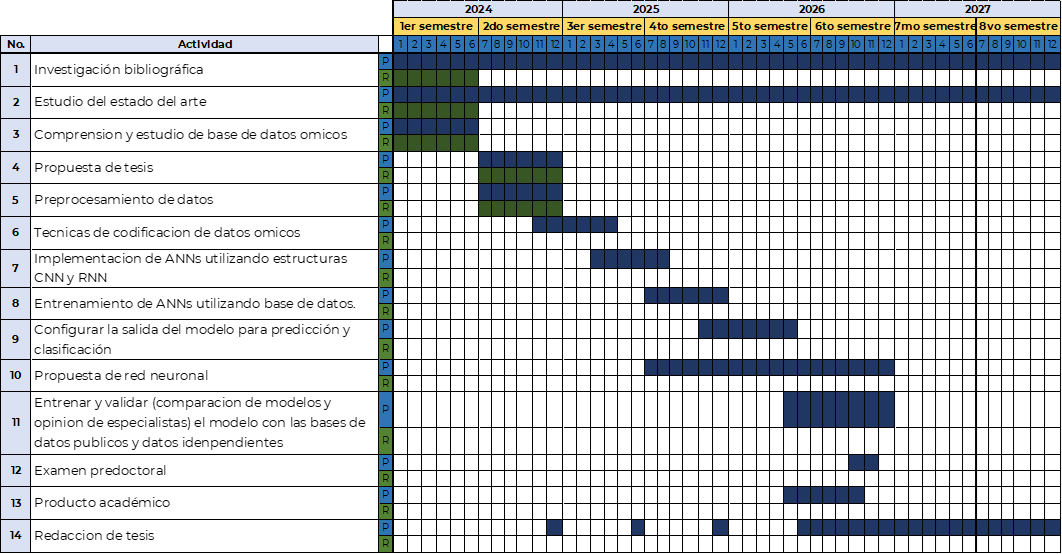
\includegraphics[width=1\textwidth]{Imagenes/Cronograma.png}
    \caption{Cronograma de actividades}\label{fig:cronograma}
\end{figure}

\newpage
\bibliographystyle{apalike} %eslito del citado %apacite %plain %apalike
\bibliography{bibliografia.bib} %archivo de las referencias

\end{document}